\documentclass{article}
\title{Sistemas Digitais e Microcontrolados - Relatório de Laboratório}
\date{}

\usepackage[utf8]{inputenc}
\usepackage[portuguese]{babel}
\usepackage[margin=3.5cm]{geometry}
\usepackage{amsmath}
\usepackage{physics}
\usepackage{titlesec}
\usepackage{graphicx}
\usepackage{wrapfig}
\usepackage{caption}
\usepackage{subcaption}
\usepackage[parfill]{parskip}
\usepackage[nottoc]{tocbibind}
\usepackage[backend=biber]{biblatex}
\addbibresource{/home/luispengler/drive/LinuxFabrik/Research/read/bib.bib}
\usepackage{authblk}
\author[1]{Jéssica Ferreira}
\author[2]{Luís Spengler}
\author[3]{Raul Lima}
\affil[1,2,3]{Instituto Federal de Educação, Ciência e Tecnologia de Mato Grosso do Sul}

\graphicspath{{./docs/}}

\begin{document}
\maketitle

\tableofcontents

\medskip

\section{Experimento 1}
\subsection{CI 7408}
O circuito integrado 7408 possui 4 portas lógicas E.

\begin{figure}[h!]
  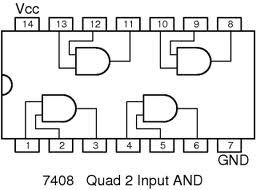
\includegraphics[scale=.7]{7408}
  \caption{7408 PINOUT}
  \label{fig:E}
\end{figure}

A tabela verdade de uma porta lógica E pode ser vista na tabela abaixo. Note que para determinarmos o correto funcionamento da CI, esta deve apresentar os mesmos resultados da tabela verdade quando medida experimentalmente.

\begin{displaymath}
\begin{array}{|c c|c|}
INPUT & & OUTPUT\\
\hline
A & B & Y\\
\hline % Put a horizontal line between the table header and the rest.
L & L & L\\
L & H & L\\
H & L & L\\
H & H & H\\
\end{array}
\end{displaymath}

Experimentalmente, ligamos INPUT nos pinos 1 e 2. OUTPUT no pino 3. Verificamos a tabela verdade da CI 7408, que usa um gate AND. Tabela obtida experimentalmente:

\begin{displaymath}
\begin{array}{|c c|c|}
INPUT & & OUTPUT\\
\hline
A & B & Y\\
\hline % Put a horizontal line between the table header and the rest.
0 & 0 & 0\\
0 & 1 & 0\\
1 & 0 & 0\\
1 & 1 & 1\\
\end{array}
\end{displaymath}

\subsection{CI 7404}
O circuito integrado 7404 possui 6 portas lógicas INVERSOR.

\begin{figure}[h!]
  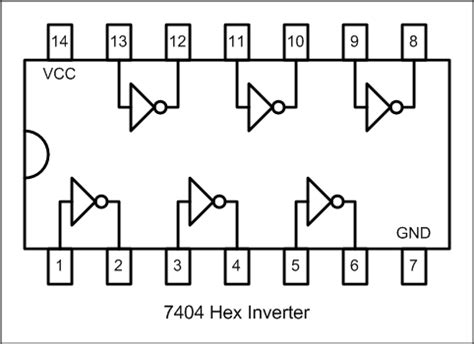
\includegraphics[scale=.7]{7404}
  \caption{7404 PINOUT}
\end{figure}

A tabela verdade de uma porta lógica INVERSOR pode ser vista na tabela abaixo. Note que para determinarmos o correto funcionamento da CI, esta deve apresentar os mesmos resultados da tabela verdade quando medida experimentalmente.

\begin{displaymath}
\begin{array}{|c c|c|}
INPUT & OUTPUT\\
\hline
A & Y\\
\hline % Put a horizontal line between the table header and the rest.
L & H\\
H & L\\
\end{array}
\end{displaymath}

Experimentalmente, ligamos INPUT no pino 3. OUTPUT no pino 4. Verificamos a tabela verdade da CI 7404, que usa um gate INVERSOR. Tabela obtida experimentalmente:

\begin{displaymath}
\begin{array}{|c c|c|}
INPUT & OUTPUT\\
\hline
A & Y\\
\hline % Put a horizontal line between the table header and the rest.
0 & 1\\
1 & 0\\
\end{array}
\end{displaymath}

\subsection{CI 7432}
O circuito integrado 7432 possui 4 portas lógicas OR.

\begin{figure}[h!]
  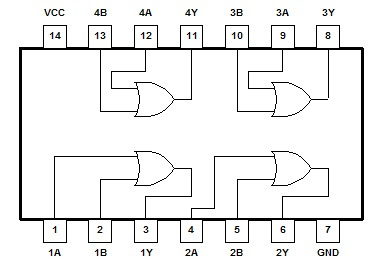
\includegraphics[scale=.7]{7432}
  \caption{7432 PINOUT}
  \label{fig:E}
\end{figure}

A tabela verdade de uma porta lógica OR pode ser vista na tabela abaixo. Note que para determinarmos o correto funcionamento da CI, esta deve apresentar os mesmos resultados da tabela verdade quando medida experimentalmente.

\begin{displaymath}
\begin{array}{|c c|c|}
INPUT & & OUTPUT\\
\hline
A & B & Y\\
\hline % Put a horizontal line between the table header and the rest.
L & L & L\\
L & H & H\\
H & L & H\\
H & H & H\\
\end{array}
\end{displaymath}

Experimentalmente, ligamos INPUT nos pinos 1 e 2. OUTPUT no pino 3. Verificamos a tabela verdade da CI 7432, que usa um gate OR. Tabela obtida experimentalmente:

\begin{displaymath}
\begin{array}{|c c|c|}
INPUT & & OUTPUT\\
\hline
A & B & Y\\
\hline % Put a horizontal line between the table header and the rest.
0 & 0 & 0\\
0 & 1 & 1\\
1 & 0 & 1\\
1 & 1 & 1\\
\end{array}
\end{displaymath}

\section{Experimento 2}
\subsection{Porta NAND}
Com o objetivo de determinar o correto funcionamento de algumas das CIs do experimento 1, utilizamos a CI 7408 (E) e a CI 7404 (OU) para a criação de uma porta NAND. Formando a seguinte tabela verdade:

\begin{displaymath}
\begin{array}{|c c|c|}
INPUT & & OUTPUT\\
\hline
A & B & Y\\
\hline % Put a horizontal line between the table header and the rest.
1 & 1 & 0\\
1 & 0 & 1\\
0 & 1 & 1\\
0 & 0 & 1\\
\end{array}
\end{displaymath}

A tabela verdade acima se assemelha com a tabela verdade de uma porta NAND, concluindo-se que sua implementação experimental foi concluida com sucesso.

\begin{displaymath}
\begin{array}{|c c|c|}
INPUT & & OUTPUT\\
\hline
A & B & Y\\
\hline % Put a horizontal line between the table header and the rest.
H & H & L\\
H & L & H\\
L & H & H\\
L & L & H\\
\end{array}
\end{displaymath}


\section{Conclusão}

Por fim, pode-se concluir que todos os gates (portas) testados experimentalmente neste relatório estavam funcionando corretamente. Até mesmo sua implementação na criação de uma porta NAND funcionou conforme esperado.

\medskip

\end{document}
